

%
\begin{enumerate}
    \item Combined sales in September and October is given by
    \begin{align}
    \vec{A}+\vec{B}=
    \begin{blockarray}{cccc}
    \text{Basmati} & \text{Permal} & \text{Naura} \\
    \begin{block}{(ccc)(c)}
    15000 & 30000 & 36000 & \text{Ram}\\
    70000 & 40000 & 20000 & \text{Guru} \\
    \end{block}
    \end{blockarray}
    \end{align}

    \item Decrease in sales from September to October is given by
    \begin{align}
    \vec{A}-\vec{B}=
    \begin{blockarray}{cccc}
    \text{Basmati} & \text{Permal} & \text{Naura} \\
    \begin{block}{(ccc)(c)}
    5000 & 10000 & 24000 & \text{Ram}\\
    30000 & 20000 & 0 & \text{Guru} \\
    \end{block}
    \end{blockarray}
    \end{align}
    
    \item Profit for sales in October is given by
    \begin{align}
    \frac{2}{100}\vec{B} =
    \begin{blockarray}{cccc}
    \text{Basmati} & \text{Permal} & \text{Naura} \\
    \begin{block}{(ccc)(c)}
    100 & 200 & 120 & \text{Ram}\\
    400 & 200 & 200 & \text{Guru} \\
    \end{block}
    \end{blockarray}
    \end{align}
    
\end{enumerate}


\begin{figure}[!ht]
\centering
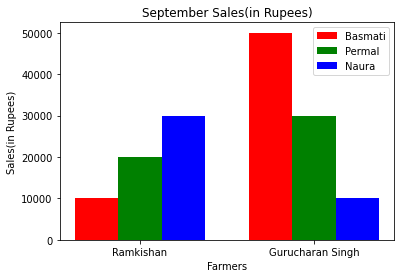
\includegraphics[width=\columnwidth]{solutions/su2021/56/Figures/Figure10_1}
\caption{September Sales(in Rupees)}
\label{matrix/56fig:SeptSales}	
\end{figure}


\begin{figure}[!ht]
\centering
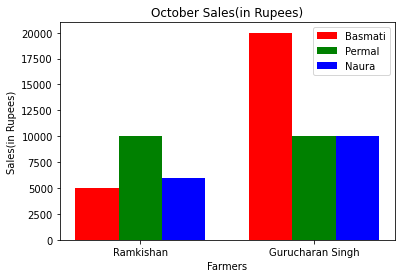
\includegraphics[width=\columnwidth]{solutions/su2021/56/Figures/Figure10_2}
\caption{October Sales(in Rupees)}
\label{matrix/56fig:OcttSales}	
\end{figure}


\begin{figure}[!ht]
\centering
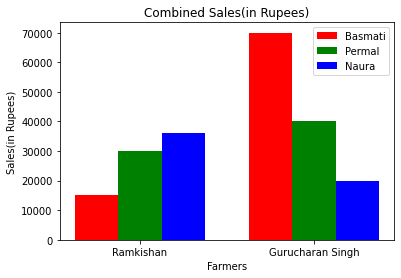
\includegraphics[width=\columnwidth]{solutions/su2021/56/Figures/Figure10_3}
\caption{Combined Sales(in Rupees)}
\label{matrix/56fig:Combined}	
\end{figure}


\begin{figure}[!ht]
\centering
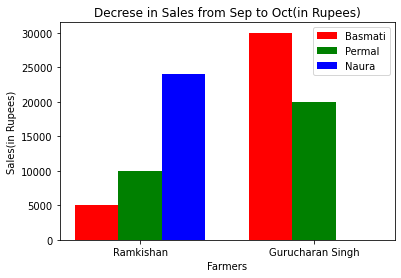
\includegraphics[width=\columnwidth]{solutions/su2021/56/Figures/Figure10_4}
\caption{Decrease in Sales from Sep to Oct(in Rupees)}
\label{matrix/56fig:Decrease}	
\end{figure}


\begin{figure}[!ht]
\centering
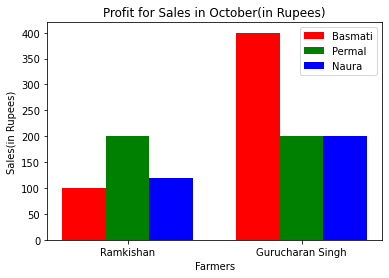
\includegraphics[width=\columnwidth]{solutions/su2021/56/Figures/Figure10_5}
\caption{Profit for Sales in October(in Rupees)}
\label{matrix/56fig:Profit}	
\end{figure}


